\documentclass{beamer}
\usepackage[utf8]{inputenc}
\usepackage[spanish]{babel}
\usepackage{graphicx}
\usepackage{adjustbox}
\usepackage{caption}
\usepackage{subcaption}
\title{Clasificación de Series de Tiempo Astronómicas}
\author{Muriel Pérez\inst{1} \and Adolfo Quiroz \inst{1} \and Alejandro García\inst{2}}
\institute[shortinst]{\inst{1} Universidad de los Andes, Departamento de Matemáticas \and%
\inst{2} Universidad de los Andes, Departamento de Física}
\begin{document}

\begin{frame}
\titlepage
\end{frame}

\begin{frame}
  \frametitle{Plan}
  \tableofcontents
\end{frame}


\section{Curvas de luz}
\begin{frame}%Mostrar una foto tomada por un telescopio y explicar como extraen las curvas de luz
  \frametitle{Curvas de Luz}
  
  \begin{figure}
    \centering
    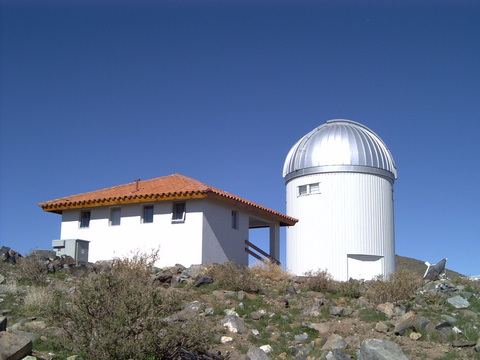
\includegraphics[width=0.8\textwidth]{./img/telescopio.jpg}
    \caption{Telescopio utilizado por el \textit{Optical Gravitational Lensing Experiment} (OGLE) localizado en Las Campanas, Chile. }
    \label{fig:gull}
  \end{figure}
\end{frame}


\begin{frame}%Mostrar curvas de luz de diferentes tipos y explicar el problema
  \frametitle{Curvas de Luz}
  \begin{figure}
    \centering
    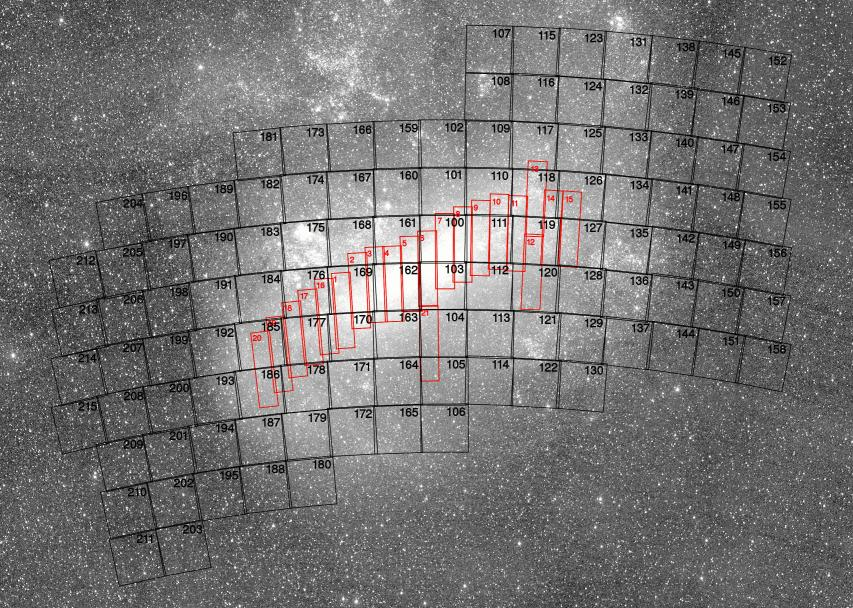
\includegraphics[width=0.8\textwidth]{./img/fields_lmc.jpg}
    \caption{Campos observados por OGLE-III en la Gran Nube de Magallanes}
    \label{fig:tiger}
  \end{figure}
\end{frame}

\begin{frame}
  \frametitle{Curvas de Luz}
  Se mide la magnitud, que está asociada a la densidad de flujo $F$ ($[F] = Wm^{-2}$) por 
  \begin{equation}
    m = -2.5\log \frac{F}{F_0}
  \end{equation} 
  \begin{figure}
    \centering
    \begin{subfigure}[b]{0.4\textwidth}
      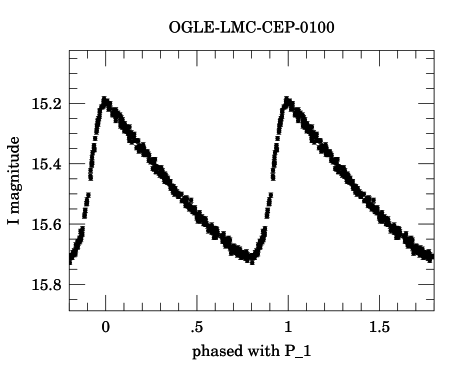
\includegraphics[width=\textwidth]{./img/OGLE-LMC-CEP-0100_1.png}
      \caption{Cefeida}
      \label{fig:gull}
    \end{subfigure}%
    ~ %add desired spacing between images, e. g. ~, \quad, \qquad, \hfill etc.
    % (or a blank line to force the subfigure onto a new line)
    \begin{subfigure}[b]{0.4\textwidth}
      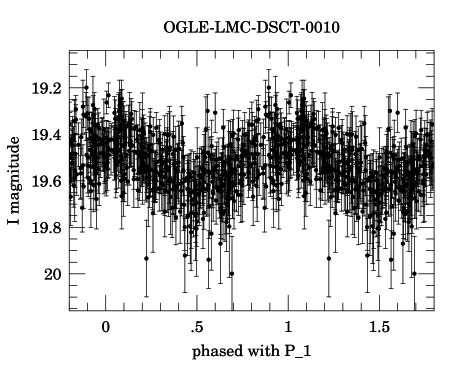
\includegraphics[width=\textwidth]{./img/OGLE-LMC-DSCT-0010_1.png}
      \caption{$\delta$-Scuti}
      \label{fig:tiger}
    \end{subfigure}
    ~ %add desired spacing between images, e. g. ~, \quad, \qquad, \hfill etc.
    % (or a blank line to force the subfigure onto a new line)
    \caption{http://www.aavso.org/types-variables}\label{fig:animals}
  \end{figure}

\end{frame}

\begin{frame}
  \frametitle{Curvas de luz}
  Con avances en instrumenación hay disponibles gran cantidad de curvas de luz. Existen proyectos como:
  \begin{itemize}
  \item Kepler Mission, NASA
  \item VISTA Variables in the Via Lactea Survey (VVV), ESO
  \item Panoramic Survey Telescope \& Rapid Response System (PANSTARRS), Universidad de Hawaii
  \end{itemize}
  Que obtendrán enetre resultados del orden de $10^9$ curvas de luz. Es necesario un sistema de clasificación automática.
\end{frame}

\begin{frame}
  \frametitle{Datos}
  
  \begin{table}
    \centering  
    \resizebox{0.6\textwidth}{!} {
      \begin{tabular}{rrr}
        \hline
        \hline
        Tipo de variabilidad y origen & \shortstack{Número \\de Objetos} & Total \\
        \hline
        \hline 
        RR Lyrae - GB\cite{soszynski_optical_2011-2} & 16836& \\
        RR Lyrae - SMC \cite{soszynski_optical_2010}& 2475&  44217\\
        RR Lyrae - LMC \cite{soszynski_optical_2009-1}& 24906& \\
        \hline
        Cefeidas - GB \cite{soszynski_optical_2011}& 32 & \\%El título del paper es classical and type2 cepheids
        Cefeidas - SMC \cite{soszynski_optical_2010-2}& 4630 & 8004\\
        Cefeidas - LMC \cite{soszynski_optical_2008-1}& 3361 & \\
        \hline
        Variables de Largo Periodo - GB \cite{soszynski_optical_2013-1}& 232406 & \\
        Variables de Largo Periodo - SMC \cite{soszynski_optical_2011-1}& 19384 & 343782\\
        Variables de Largo Periodo -  LMC\cite{soszynski_optical_2009}& 91995 & \\
        \hline
        Binarias Eclipsantes - SMC \cite{pawlak_eclipsing_2013}& 6138 & 32259\\
        Binarias Eclipsantes - LMC \cite{graczyk_optical_2011}& 26121 & \\
        \hline
        $\delta$-Scuti - SMC\cite{poleski_optical_2010} & 2786 & 2788\\
        \hline
        Cefeidas Tipo II - GB \cite{soszynski_optical_2013}& 335 & \\
        Cefeidas Tipo II - LMC \cite{soszynski_optical_2010-1}& 43 & 603\\
        Cefeidas Tiplo II - LMC \cite{soszynski_optical_2008}& 197 & \\
        \hline
        Cadidatas a Be -  Vía Láctea  & 475 & 475\\
        \hline
        \hline 
      \end{tabular}
    } 
    \caption{Conjunto de datos utilizados. GB hace referencia al Bulbo Galáctico; LMC, a la Pequeña Nube de Magallanes y LMC, a la Gran Nube de Magallanes. }
    \label{cuadro:datosUsados}
  \end{table}

\end{frame}

\begin{frame}
  \frametitle{Tipos de Variabilidad}
  En esta diapositiva va una curva de luz de cada tipo.
\end{frame}


\section{El problema de aprendizaje}
\begin{frame}%Caracteristicas
  \frametitle{Características}
\begin{itemize}
   \item Cada curva de luz es un objeto complicado (diferentes números de mediciones hechas en intervalos irregulares de tiempo).  
   \item A cada curva de luz podemos asignarle un vector $\vec{x}_i\in\mathbb{R}^n$ de cantidades calculadas a partir de los valores de magnitud y los instantes en que fueron medidos. Cada uno de esos vectores tiene una etiqueta $j\in J = \{RR Lyrae,..., Be\}$, que corresponde al tipo de variabilidad de la estrella observada.
     \item El vector $\vec{x}_i\in\mathbb{R}^n$  es llamado vector de características.
\end{itemize}
\end{frame}

\begin{frame}
  Aquí va una curva de luz con su histograma
\end{frame}

\begin{frame}
  Debido a que en algunas curvas existen puntos atípicos, es necesario utilizar medidas robustas. Estas medidas están típicamente basadas en cuantiles de la distribución de las magniudes. 
  Aquí va una curva de luz con un punto atípico
\end{frame}

\subsection{Características Escogidas}
\begin{frame}
\frametitle{Caracteristicas escogidas}
Las medidas escogidas debían ser robustas ante la presencia de datos atípicos.
\begin{table}
  \centering
  \begin{tabular}{ll}
    \hline
    Variables de localización & Media \\
    \hline
    Variables de escala & Rango Intercuartiles (IQR) \\
    & Desviación Absoluta Mediana (MAD) \\
    Medidas de Sesgo & \textit{Medcouple} \\
    & Medidas de peso de colas \\
    Medidas de forma & Entropía diferencial \\
    & Valores Abbe \\
  \end{tabular}
  \caption{Varriables escogidas}
\end{table}

\end{frame}

\begin{frame}
  \frametitle{Parámetros de Escala}
  La desviación estándar muestral es sensible a la presencia de puntos atípicos. Utilizamos la desviación absuluta mediana (MAD)
  \begin{equation}
    \sigma = mediana_i(|m_i-mediana_j(m_j)|).
  \end{equation} 
  Y el rango intercuartiles (IQR)
  \begin{equation}
    IQR = Q_{0.75}-Q_{0.25}
  \end{equation}
\end{frame}

\begin{frame}
  \frametitle{Parámetros de Localización}
  Utilizamos un estimador robusto del promedio que hace parte de los llamados M-estimadores. Huber propuso escoger $\mu$ al resolver resolver el problema 
  \begin{equation}
    \sum_i\psi\left(\frac{m_i-\mu}{\sigma}\right) = 0
  \end{equation}
  donde $\sigma$ es la MAD y 
  \begin{equation}
    \psi(x) = \begin{cases} 
      -c &\mbox{si } x < -c \\ 
      x & \mbox{si } |x|<c\\
      c & \mbox{si } x>c
    \end{cases}
  \end{equation}
\end{frame}

\begin{frame}
  \frametitle{Medidas de Sesgo}
  Para calcular el sesgo es necesario calcular $(m_i-\mu)^3$ por lo que es sensible a la presencia de datos atípicos. Utilizamos medidas de sesgo de la forma 
  \begin{equation}
    \frac{(Q_{1-p}-Q_{0.5})-(Q_{0.5}-Q_p)}{Q_{1-p}-Q_{p}}
  \end{equation}
  para p = 0.125, 0.25. Además consideramos el \textit{medcouple}
  \begin{equation}
    MC = mediana_{x_i\leq Q_{0.5} x_j} h_1(x_i,x_j)
  \end{equation}
  con
  \begin{equation}
    h_1(x_i,x_j) = \frac{(x_{(j)}-Q_{0.5})-(Q_{0.5}-x_{(i)})}{x_{(j)}-x_{(i)}}
  \end{equation}

\end{frame}

\begin{frame}
  \frametitle{Entropía Diferencial}
  Utilizamos un estimado de la densidad $f$ por núcleos $\hat{f}$ de las magnitudes que se encuentren entre la mediana y $\pm 6\sigma$ y estimamos la entropía diferencial 
  \begin{equation}
    H(M) = -\int f(m)\log f(m) dm
  \end{equation}
  con 
  \begin{equation}
    \hat{H}(M) \approx -\frac{1}{n}\sum_i\log\hat{f}(m_i)
  \end{equation}
\end{frame}

\begin{frame}
  \frametitle{Valor Abbe}
  El valor Abbe fue propuesto por (cita) para detectar curvas de luz con fenómenos transientes. Se define como
  \begin{equation}
    \mathcal{A}=\frac{n}{2(n-1)}\frac{\sum_{i}{(m_{i}-m_{i-1})^{2}}}{\sum_{i}{(m_{i}-\mu})^2}
  \end{equation}
  y puede ser calculado en subintervalos de tiempo.
\end{frame}

\subsection{Aprendizaje supervisado}
\begin{frame}%Poner aqui el problema en general encontrar una funci g tq ta ta ta
\frametitle{Clasificadores}
El problema: Encontrar una función $g:\mathbb{R}^n\to J  $ que se equivoque lo menos posible.
\begin{itemize}
  \item Suponemos que hay una medida de probabilidad $P$ sobre $\mathbb{R}^n\times J$ tal que $P(\vec{x}, j)$ es la probabilidad de observar el vector $\vec{x}$ con la etiqueta $j$.
  \item La probabilidad de que nuestro clasificador $g$ se equivoque es $P(g(\vec{x}) \neq j)$. Queremos maximizar $P(g(\vec{x}) = j)$.
  \end{itemize}
\end{frame}


\subsection{Clasificador de Bayes}
\begin{frame}%Explicar cual es el mejor clasificador posible
  \frametitle{El clasificador de Bayes}
  ¿Cuál es el mejor clasificador posible?
  \begin{itemize} 
  \item El clasificador
    \begin{equation}
      g(\vec{x}) = argmax_{j}P(\vec{x}|j)P(j)
    \end{equation}
    es llamado el \textbf{clasificador de Bayes}. Es el mejor clasificador posible.
  \end{itemize}
  En general no se conocen las distribuciones marginales $P(\vec{x}|j)$.
\end{frame}

\subsection{Metodología de Aprendizaje}
\begin{frame} %Hablar de el proceso de entrenamiento
  \frametitle{Metodología de aprendizaje}
  \begin{itemize}
  \item Utilizamos un \textbf{algorítmo de aprendizaje} para escoger una regla de clasificación de un \textbf{conjunto de hipótesis}.
  \item Estimamos el error de clasificación usando \textbf{validación cruzada} de 10 iteraciones.
  \end{itemize}
\end{frame}


\subsection{Clasificadores y Resultados}
\begin{frame}%k vecinos más cercanos
  \frametitle{k Vecinos Más Cercanos}
A un punto a clasificar se la asigna la clase a la cual pertenece la mayoría entre sus k vecinos más cercanos. Se sabe que este método es consistente, es decir, que tiende al clasificador de Bayes cuando el tamaño de la muestra tiende a infinito. Existe una implementación abierta en el paquete FNN para R.

    \begin{table}[ht]
      \centering
  \resizebox{0.7\textwidth}{!} {
      \begin{tabular}{rrrrrrrr}
        \hline
        \hline
        Referencia& BeEC & Cef & dSct & SBE & VLP & RRLyr & CefT2 \\ 
        \hline
        \hline
        BeEC & 0.762 & 0.001 & 0.000 & 0.001 & 0.000 & 0.000 & 0.002 \\ 
        Cef & 0.061 & 0.832 & 0.004 & 0.005 & 0.000 & 0.041 & 0.166 \\ 
        dSct & 0.000 & 0.001 & 0.648 & 0.014 & 0.000 & 0.010 & 0.000 \\ 
        SBE & 0.080 & 0.016 & 0.175 & 0.915 & 0.001 & 0.027 & 0.078 \\ 
        VLP & 0.076 & 0.007 & 0.003 & 0.022 & 0.998 & 0.001 & 0.090 \\ 
        RRLyr & 0.021 & 0.139 & 0.169 & 0.041 & 0.000 & 0.920 & 0.289 \\ 
        CefT2 & 0.000 & 0.004 & 0.000 & 0.001 & 0.000 & 0.002 & 0.376 \\ 
        \hline
        \hline
        Sensitividad & 0.762 & 0.832 & 0.648 & 0.915 & 0.998 & 0.920 & 0.376 \\ 
        \hline
        Error & 0.038 & 0.008 & 0.018 & 0.003 & 0.000 & 0.003 & 0.039 \\ 
        \hline
        \hline
      \end{tabular}
    }
    \end{table}
\end{frame}

\begin{frame}
  \frametitle{Árboles de clasificación}
  Fue propuesta por Breiman, Friedman, Stone y Olshen (cita). Creamos un árbol de decisión para clasificar los datos. Para clasificar un nuevo dato se hacen preguntas binarias de tipo $x_i\leq \alpha_i$. Si la respuesta es sí se procede al siguiente nodo de la izquierda y si es no,  a la derecha. En los nodos terminales se le asigna al nuevo dato una etiqueta. 
  
  Existe una implementación libre en el paquete rpart para R.


  \begin{table}[ht]
    \centering
    \resizebox{0.7\textwidth}{!} {
      \begin{tabular}{rrrrrrrr}
        \hline
        & BeEC & Cef & dSct & SBE & VLP & RRLyr & CefT2 \\ 
        \hline
        BeEC & 0.903 & 0.008 & 0.002 & 0.026 & 0.007 & 0.001 & 0.005 \\ 
        Cef & 0.038 & 0.824 & 0.005 & 0.009 & 0.041 & 0.259 & 0.214 \\ 
        dSct & 0.000 & 0.003 & 0.907 & 0.165 & 0.000 & 0.079 & 0.002 \\ 
        SBE & 0.002 & 0.011 & 0.054 & 0.624 & 0.000 & 0.034 & 0.020 \\ 
        VLP & 0.011 & 0.013 & 0.009 & 0.058 & 0.890 & 0.002 & 0.005 \\ 
        RRLyr & 0.000 & 0.002 & 0.022 & 0.002 & 0.000 & 0.509 & 0.007 \\ 
        CefT2 & 0.046 & 0.139 & 0.002 & 0.116 & 0.060 & 0.116 & 0.748 \\ 
        \hline
        \hline
        Sensitividad & 0.903 & 0.824 & 0.907 & 0.624 & 0.890 & 0.509 & 0.748 \\ 
        \hline
        Error & 0.027 & 0.008 & 0.011 & 0.005 & 0.001 & 0.005 & 0.035 \\ 
        \hline
        \hline
      \end{tabular}
    }
  \end{table}
\end{frame}


\begin{frame}
  \frametitle{Bosques aleatorios}
  Fue propuesto por Breiman (cita). Se crean árboles de clasificación que son clasificadores débiles pero que están poco correlacionados. Se toma la decisión utilizando la regla de la mayoría. Los árboles son creados utilizando un subconjunto aleatorio de las características en cada nodo y solo se construyen árboles poco profundos.
  \begin{table}[ht]
    \centering
    \resizebox{0.7\textwidth}{!} {
      \begin{tabular}{rrrrrrrr}
        \hline
        Referencia & BeEC & Cef & dSct & SBE & VLP & RRLyr & CefT2 \\ 
        \hline
        BeEC & 0.842 & 0.000 & 0.000 & 0.000 & 0.000 & 0.000 & 0.000 \\ 
        Cef & 0.002 & 0.810 & 0.002 & 0.001 & 0.000 & 0.018 & 0.138 \\ 
        dSct & 0.000 & 0.000 & 0.738 & 0.004 & 0.000 & 0.004 & 0.000 \\ 
        SBE & 0.103 & 0.013 & 0.146 & 0.959 & 0.000 & 0.014 & 0.108 \\ 
        VLP & 0.048 & 0.009 & 0.004 & 0.020 & 1.000 & 0.001 & 0.111 \\ 
        RRLyr & 0.004 & 0.166 & 0.110 & 0.016 & 0.000 & 0.963 & 0.299 \\ 
        CefT2 & 0.000 & 0.002 & 0.000 & 0.000 & 0.000 & 0.000 & 0.345 \\
        \hline
        \hline
        Sensitividad &  0.842 & 0.810 & 0.738 & 0.959 & 1.000 & 0.963 & 0.345 \\
        \hline
        Error & 0.033 & 0.009 & 0.016 & 0.002 & 0.000 & 0.002 & 0.038 \\ 
        \hline
        \hline
      \end{tabular}
    }
  \end{table}
\end{frame}



\begin{frame}
\frametitle{Máquinas de Soporte Vectorial (SVM)}
Consideremos un problema de dos clases, es decir, $J=\{-1,1\}$. Queremos una regla de decisión 
\begin{equation}
g(\vec{x}) = sign(\langle \vec{w}, \vec{x}\rangle + b)
\end{equation}
que maximice la distancia de los puntos al plano perpendicular a $\vec{w}$
En el caso en que los datos sean linealmente separables, podemos encontrar el plano resolviendo el problema de optimización
\begin{equation*}
\begin{aligned}
& \underset{\vec{w}}{\text{minimizar}}
& & \langle \vec{w}, \vec{w} \rangle \\
& \text{sujeto a}
& & j_i(\langle \vec{w}, \vec{x_i}\rangle + b)\geq 1, \; i = 1, \ldots, N.
\end{aligned}
\end{equation*}
\end{frame}


\begin{frame}
\frametitle{Máquinas de Soporte Vectorial (SVM)}
Si los datos no son linealmente separables, podemos introducir variables de holgura $\xi_i$ y resolver
\begin{equation*}
\begin{aligned}
& \underset{\alpha}{\text{minimizar}}
& & \langle \vec{w}, \vec{w}\rangle + C\sum_i\xi_i  \\
& \text{sujeto a}
& & j_i(\langle \vec{w}, \vec{x_i}\rangle + b)\geq 1-\xi_i, \; i = 1, \ldots, N.\\
& & & \xi_i\geq 0 \; i = 1, \ldots, N.
\end{aligned}
\end{equation*} 
cuyo problema dual es
\begin{equation*}
\begin{aligned}
& \underset{\alpha}{\text{minimizar}}
& & \frac{1}{2} \sum_{i,k} j_{i}j_{k}\alpha_{i}\alpha_{k}\langle \vec{x}_{i}, \vec{x}_{k}\rangle - \sum_{i} \alpha_{i}  \\
& \text{sujeto a}
& & \sum_{i}\alpha_{i} j_{i} = 0\\
& & & 0\leq\alpha_i\leq C \; i = 1, \ldots, N.
\end{aligned}
\end{equation*}
\end{frame} 


\begin{frame}
\frametitle{Máquinas de Soporte Vectorial (SVM)}
El problema de optimización solo depende de la matriz $\langle \vec{x}_i, \vec{x}_j\rangle$. Podemos encontrar una función $K(\vec{x}, \vec{y})$ que cumpla $K(\vec{x}, \vec{y}) = \langle \phi(\vec{x}) , \phi(\vec{y})\rangle_{H}$ para cierta función $\phi:\mathbb{R}^n\rightarrow H$ siendo $H$ algún espacio con producto interno y encontrar el plano separador en $H$ resolviendo el problema de optimización.
\begin{equation*}
\begin{aligned}
& minimizar
& & \frac{1}{2} \sum_{i,k} j_{i}j_{k}\alpha_{i}\alpha_{k}K( \vec{x}_{i}, \vec{x}_{k}) - \sum_{i} \alpha_{i}  \\
& \text{sujeto a}
& & \sum_{i}\alpha_{i} j_{i} = 0\\
& & & 0\leq\alpha_i\leq C \; i = 1, \ldots, N.
\end{aligned}
\end{equation*}
\end{frame}

\begin{frame}
\frametitle{Máquinas de Soporte Vectorial}
  \begin{table}[ht]
    \centering
    \resizebox{0.7\textwidth}{!} {
      \begin{tabular}{rrrrrrrr}
        \hline
        Referencia & BeEC & Cef & dSct & SBE & VLP & RRLyr & CefT2 \\ 
        \hline
        BeEC & 0.891 & 0.000 & 0.000 & 0.001 & 0.000 & 0.000 & 0.000 \\ 
        Cef & 0.002 & 0.869 & 0.002 & 0.002 & 0.000 & 0.016 & 0.128 \\ 
        dSct & 0.000 & 0.000 & 0.769 & 0.006 & 0.000 & 0.005 & 0.002 \\ 
        SBE & 0.048 & 0.008 & 0.117 & 0.963 & 0.001 & 0.013 & 0.075 \\ 
        VLP & 0.053 & 0.004 & 0.005 & 0.016 & 0.999 & 0.001 & 0.070 \\ 
        RRLyr & 0.006 & 0.115 & 0.107 & 0.012 & 0.000 & 0.964 & 0.265 \\ 
        CefT2 & 0.000 & 0.004 & 0.000 & 0.001 & 0.000 & 0.001 & 0.461 \\
        \hline
        \hline
        Sensitividad &  0.891 & 0.869 & 0.769 & 0.963 & 0.999 & 0.964 & 0.461 \\ 
        \hline
        Error & 0.028 & 0.007 & 0.016 & 0.002 & 0.000 & 0.002 & 0.040 \\ 
        \hline
        \hline
      \end{tabular}
    }
  \end{table}
\end{frame}

\begin{frame}
\frametitle{Conclusiones}
En esta diapositiva va un diagrama de barras con cada una de las sensitividades por clase y por método. También sus especificidades.
\end{frame}

\begin{frame}
\frametitle{conclusiones}
Maravillosa frase final
\end{frame}

\begin{frame}[allowframebreaks]
  \frametitle{Referencias}
  \bibliographystyle{plain}
  \bibliography{tesisMatematicas,rPackagesCitations}
\end{frame}

\end{document}
